\chapter{Matrix constructions}
\label{chap_matrix_examples}
\textsf{In this chapter, we will see a few examples of modified block-Toeplitz matrices, as well as the vector representation.}

\section{The block-Toeplitz matrix} 
\label{sec_toeplitz}
Let's consider the term:
\begin{equation}
T=\sum_{c_x}\sum_{c_y}M_{i-c_x,j-c_y}C_{c_x,c_y}
\label{eq_convolution}
\end{equation}
which is a convolution between the space harmonics representing $\mu_x$ and those representing $H_y$. We notice that this term comes directly from the product $\mu_x H_y$, and this is a direct consequence of the well known convolution theorem for Fourier transforms.

The first problem we have to face is that up to now, the Fourier expansion has been done by using an infinite number of harmonics. We thus need to truncate the series to a finite number of terms. We will call $S_x$ and $S_y$ the number of positive and negative coefficients considered in $x$ and $y$. The infinite sum of the convolution~\eqref{eq_convolution} thus becomes finite:
\begin{equation}
T'_{i,j}=\sum_{c_x=-(S_x-1)}^{(S_x-1)}\sum_{c_y=-(S_y-1)}^{(S_y-1)}M_{i-c_x,j-c_y}C_{c_x,c_y}
\label{eq_finiteconvolution}
\end{equation}
We now want to write it as a matrix-vector product:
\begin{equation}
T'=\dbar{M} \bar{C}
\end{equation}
To obtain this, we can unroll the $x$ and $y$ components of the $C_{c_x,c_y}$ space harmonics in order to write the vector $\bar{C}$ as follows:
\begin{equation}
\bar{C}=
\begin{pmatrix}
C_{-(S_x-1),-(Sy-1)}\\
C_{-(S_x-2),-(S_y-1)}\\
C_{-(S_x-3),-(S_y-1)}\\
\cdots\\
C_{S_x-1,-(S_y-1)}\\
C_{-(S_x-1),-(Sy-2)}\\
\cdots\\
C_{-(S_x-1),0}\\
C_{-(S_x-2),0}\\
\cdots\\
C_{-1,0}\\
C_{0,0}\\
C_{1,0}\\
\cdots\\
C_{(S_x-1),(Sy-1)}\\
\end{pmatrix}
\end{equation}
This vector can be assembled by rearranging the coefficients of the $(2S_y-1)\times(2S_x-1)$ Fourier matrix:  
\begin{equation}
\dbar{C}=
\begin{pmatrix}
C_{0,0}     	& C_{1,0}			&\cdots	& C_{S_x-1,0}	& \cdots& C_{-1,0}\\
C_{0,1}     	& C_{1,1}			&		&				&		& \\
C_{0,2}     	& C_{1,2}			&		&				&		& \\
\cdots      	& \cdots			&		&				&		& \\
C_{0,S_y-1} 	& C_{1,S_y-1}		& 	    &				&       & \\
C_{0,-(S_y-1)} 	& C_{1,-(S_y-1)} 	&		&				&		& \\
C_{0,-(S_y-2)} 	& C_{1,-(S_y-2)} 	&		&				&		& \\
\cdots			& \cdots			&		&				&		& \\
C_{0,-1}		& C_{1,-1}			&		&	\cdots		&		& C_{-1,-1}
\cdots\\
\end{pmatrix}
\end{equation}
Which is the usual form in which the results of a 2D FFT algorithm are stored.\footnote{Note that in usual matrix notation $A_{i,j}$ means the $i$-row and $j$-column, while we want to maintain a strong relationship with space coordinates.}
The matrix $\dbar{M}_\indT$ can be constructed from $M_{i,j}$ as a block-Toeplitz matrix. We will use the notation $\dbar{M}_\indT$ to stress that this is a block-Toeplitz matrix built from the $M_{i,j}$ Fourier coefficients:
\begin{equation}
\dbar{M}_\indT=
\begin{pmatrix}
\dbar{T}_{0} & \dbar{T}_{-1} & \dbar{T}_{-2} & \cdots \\
\dbar{T}_{1} & \dbar{T}_{0} & \dbar{T}_{-1} & \cdots \\
\dbar{T}_{2} & \dbar{T}_{1} & \dbar{T}_{0} & \cdots \\
\cdots\\
\label{eq_block_toeplitz1}
\end{pmatrix}
\end{equation}
in which each block $\dbar{T}_j$ can be written as follows:
\begin{equation}
\dbar{T}_j=
\begin{pmatrix}
M_{0,j} & M_{-1,j} & M_{-2,j} & \cdots \\
M_{1,j} & M_{0,j} & M_{-1,j} & \cdots \\
M_{2,j} & M_{1,j} & M_{0,j} & \cdots \\
\cdots\\
\label{eq_block_toeplitz2}
\end{pmatrix}
\end{equation}
An example of construction of such a matrix is given in section~\ref{sec_block_toeplitz_examples}.
The size of the (square) $\dbar{M}_\indT$ matrix\footnote{If we take $S_x$ space harmonics, this gives us $2S_x+1$ Fourier coefficient. We can compute only $S_x$ Fourier terms of the result of the convolution, thus giving a matrix size of $(S_x S_y)\times (S_x S_y)$.} is thus $(S_x S_y)\times (S_x S_y)$.

\section[The modified Toeplitz notation]{Representing derivatives: the modified Toeplitz notation}
\label{sec_derivatives}
In equations describing field propagation, we can find complex convolutions, like the following one:
\begin{equation}
T_{i,j}=\sum_{d_x}\sum_{d_y}R_{i-d_x,j-d_y}(\junit)(j-d_y)\nu_y D_{d_x,d_y}(\junit d_x\nu_x)
\end{equation}
which in the Fourier base represents the term:
\begin{equation}
\frac{\partial}{\partial y}\frac{1}{\junit \omega\epsilon_z} \frac{\partial H_y}{\partial x}
\end{equation}
A difference from the convolution \eqref{eq_convolution} is that there is a multiplication of each term $D_{d_x,d_y}$ by the constant $(\junit d_x\nu_x)$. This is given by the $x$ derivative of $H_y$. We have also  $R_{i-d_x,j-d_y}$ multiplied by the term $(\junit)(j-d_y)\nu_y$, which comes from the $y$ derivative of $\epsilon_z^{-1}$, as we have seen in section~\ref{sec_toeplitz}.
We want to write this convolution in a compact matrix by vector product:
\begin{equation}
T''=\dbar{R}_{\indT y}^{(x)} \bar{D}
\end{equation}
where the $\bar{D}$ vector is built as usual from the $D_{i,j}$ Fourier components.
The shorthand notation $\dbar{R}_{\indT y}^{(x)}$ means that we have taken into account in the construction of the matrix some products coming from the derivatives. This can be obtained by using the Hadamard product of the block-Toeplitz matrix by two matrices $\mathcal{C}_y$ and $\mathcal{C}^{(x)}$, which contain the multiplication terms coming from derivatives:
\begin{equation}
\dbar{R}_{\indT y}^{(x)}=\dbar{R}_\indT \bullet \mathcal{C}_y \bullet \mathcal{C}^{(x)}
\end{equation}
The first matrix $\mathcal{C}_y$ is the block-Toeplitz matrix built with space harmonics:
\begin{equation}
\mathcal{C}_y=
\begin{pmatrix}
	T_{0} & T_{-1} & T_{-2} & \cdots \\
	T_{1} & T_{0} & T_{1} & \cdots \\
	T_{2} & T_{1} & T_{0} & \cdots \\
\cdots\\
\end{pmatrix}
\end{equation}
in which each block $T_j$ is a constant matrix:
\begin{equation}
\dbar{T}_j=
\begin{pmatrix}
j\nu_y & j\nu_y & j\nu_y & \cdots \\
j\nu_y & j\nu_y & j\nu_y & \cdots \\
j\nu_y & j\nu_y & j\nu_y & \cdots \\
\cdots\\
\end{pmatrix}
\end{equation}

The matrix $\mathcal{C}^{(x)}$ is made by $(S_x S_y)$ identical columns containing multiples of the fundamental space frequency arranged in the same order used during the construction of the block-Toeplitz matrix $M_\mathrm{T}$ seen above.
The section~\ref{sec_modified_toeplitz_examples} presents a few examples of construction of small size $\mathcal{C}$ matrices.

We will call the matrix $\dbar{R}_{\indT y}^{(x)}$ a modified block-Toeplitz matrix.
This type of notation is completely general and will allow us to write  matrix equations directly and quickly from equations in the original space. To represent in the finite size Fourier base products and derivatives, one has simply to write the corresponding modified block-Toeplitz matrix.\footnote{Please note that the multiplication times the $\junit$ imaginary unit coming from the derivatives is not taken into account in the matrix construction and should be done explicitly.}

\section{Unrolling vectors}
The first difficulty encountered in treating the 2D problem is that we need to store in a vector way the 2D set of space harmonics. The usual representation given for example by a standard 2D FFT stores the harmonics in a matrix. In our examples, we will consider a $5\times 5=(2S_y-1)\times(2S_x-1)$ matrix size in which the real part of each element gives the the $x$ harmonic order, while the imaginary part gives  the  $y$ harmonic order. In the real case, this will be used for the calculation of the Fourier transform by means of a FFT or an analytically calculated Fourier transform, but this will allow us to develop the examples for the following more complex constructions. Let's see an example:
\begin{equation}
\dbar{A} =
\begin{pmatrix}
0		   &	1	    &	2		   &-2		    &  -1       \\
\junit   & 1+\junit  	&	2+\junit   &-2+\junit  	&-1+\junit  \\
2\junit  & 1+2\junit  &	2+2\junit  &-2+2\junit  &-1+2\junit  \\
-2\junit  & 1-2\junit  &	2-2\junit  &-2-2\junit  &-1-2\junit  \\
-1\junit  & 1-1\junit  &	2-1\junit  &-2-1\junit  &-1-1\junit  
\end{pmatrix}
\end{equation}
In our case, we obtain $S_x=3$ and $S_y=3$, which means that we are considering three space harmonics, including the zero-order (continuous) term.
Unrolling the $\dbar{A}$ matrix gives us the $\bar{A}$ vector:
\begin{equation}
\begin{aligned}
\bar{A}=
(-2-2\junit, -1-2\junit, -2\junit, 1-2\junit, 2-2\junit, \\
-2-\junit, -1-\junit, 0-\junit, 1-\junit, 2-\junit, \\
-2, -1, 0, 1, 2,
-2+\junit, -1+\junit, \junit, 1+\junit, 2+\junit, \\
-2+2\junit, -1+2\junit, 2\junit, 1+2\junit, 2+2\junit)^\mathrm{T}
\end{aligned}
\end{equation}
where $\mathrm{T}$ means the transpose operation to obtain a column vector.

\section{Creating bloc-Toeplitz matrix}
\label{sec_block_toeplitz_examples}
We can write the corresponding Bloc-Toeplitz matrix for the vector $\bar{A}$. The multiplication of that matrix for an unrolled vector $\bar{B}$ will result in the convolution in the Fourier domain between the space harmonics of the two vectors. This typically represent a simple multiplication in the original space.
The $\dbar{A}$ matrix will have a $S_xS_y\times S_xS_y$ size, which in our example is $9\times 9$. 

The bloc-Toeplitz matrix in our case is the following one:
{\footnotesize
\begin{equation}
\dbar{A}_\mathrm{T}=
\begin{pmatrix}
  0 + 0\junit & -1 + 0\junit&  -2 + 0\junit &  0 - 1\junit & -1 - 1\junit & -2 - 1\junit &  0 - 2\junit & -1 - 2\junit & -2 - 2\junit \\
   1 + 0\junit &  0 + 0\junit & -1 + 0\junit &  1 - 1\junit &  0 - 1\junit & -1 - 1\junit &  1 - 2\junit &  0 - 2\junit & -1 - 2\junit \\
   2 + 0\junit &  1 + 0\junit &  0 + 0\junit &  2 - 1\junit &  1 - 1\junit &  0 - 1\junit &  2 - 2\junit &  1 - 2\junit &  0 - 2\junit\\
   0 + 1\junit & -1 + 1\junit & -2 + 1\junit &  0 + 0\junit & -1 + 0\junit & -2 + 0\junit &  0 - 1\junit & -1 - 1\junit & -2 - 1\junit\\
   1 + 1\junit &  0 + 1\junit & -1 + 1\junit &  1 + 0\junit &  0 + 0\junit & -1 + 0\junit &  1 - 1\junit &  0 - 1\junit & -1 - 1\junit\\
   2 + 1\junit &  1 + 1\junit &  0 + 1\junit &  2 + 0\junit &  1 + 0\junit &  0 + 0\junit &  2 - 1\junit &  1 - 1\junit &  0 - 1\junit\\
   0 + 2\junit & -1 + 2\junit & -2 + 2\junit &  0 + 1\junit & -1 + 1\junit & -2 + 1\junit &  0 + 0\junit & -1 + 0\junit & -2 + 0\junit\\
   1 + 2\junit &  0 + 2\junit & -1 + 2\junit &  1 + 1\junit &  0 + 1\junit & -1 + 1\junit &  1 + 0\junit &  0 + 0\junit & -1 + 0\junit\\
   2 + 2\junit &  1 + 2\junit &  0 + 2\junit &  2 + 1\junit &  1 + 1\junit &  0 + 1\junit &  2 + 0\junit &  1 + 0\junit &  0 + 0\junit
\end{pmatrix}
\end{equation}
}
The modification matrices $\mathcal{C}_x$ and $\mathcal{C}_y$ are the following ones :
\begin{equation}
\mathcal{C}_x= \nu_x
\begin{pmatrix}
   0 & -1 & -2 &  0 & -1 & -2 &  0 & -1 & -2\\
   1 &  0 & -1 &  1 &  0 & -1 &  1 &  0 & -1\\
   2 &  1 &  0 &  2 &  1 &  0 &  2 &  1 &  0\\
   0 & -1 & -2 &  0 & -1 & -2 &  0 & -1 & -2\\
   1 &  0 & -1 &  1 &  0 & -1 &  1 &  0 & -1\\
   2 &  1 &  0 &  2 &  1 &  0 &  2 &  1 &  0\\
   0 & -1 & -2 &  0 & -1 & -2 &  0 & -1 & -2\\
   1 &  0 & -1 &  1 &  0 & -1 &  1 &  0 & -1\\
   2 &  1 &  0 &  2 &  1 &  0 &  2 &  1 &  0
\end{pmatrix}
\end{equation}
\begin{equation}
\mathcal{C}_y= \nu_y
\begin{pmatrix}
   0 &  0 &  0 & -1 & -1 & -1 & -2 & -2 & -2\\
   0 &  0 &  0 & -1 & -1 & -1 & -2 & -2 & -2\\
   0 &  0 &  0 & -1 & -1 & -1 & -2 & -2 & -2\\
   1 &  1 &  1 &  0 &  0 &  0 & -1 & -1 & -1\\
   1 &  1 &  1 &  0 &  0 &  0 & -1 & -1 & -1\\
   1 &  1 &  1 &  0 &  0 &  0 & -1 & -1 & -1\\
   2 &  2 &  2 &  1 &  1 &  1 &  0 &  0 &  0\\
   2 &  2 &  2 &  1 &  1 &  1 &  0 &  0 &  0\\
   2 &  2 &  2 &  1 &  1 &  1 &  0 &  0 &  0
\end{pmatrix}
\end{equation}

These terms represent in the Fourier space the $x$ and $y$ derivative of the first term of the product in the original space.

The modification matrices $\mathcal{C}^{(x)}$ and $\mathcal{C}^{(y)}$ are the following ones (for $\nu_x=\nu_y=1$):
\begin{equation}
\mathcal{C}^{(x)}=\nu_x
\begin{pmatrix}
-1 &0 &1 &-1 &0 &1 &-1 &0 &1 \\
-1 &0 &1 &-1 &0 &1 &-1 &0 &1 \\
-1 &0 &1 &-1 &0 &1 &-1 &0 &1 \\
-1 &0 &1 &-1 &0 &1 &-1 &0 &1 \\
-1 &0 &1 &-1 &0 &1 &-1 &0 &1 \\
-1 &0 &1 &-1 &0 &1 &-1 &0 &1 \\
-1 &0 &1 &-1 &0 &1 &-1 &0 &1 \\
-1 &0 &1 &-1 &0 &1 &-1 &0 &1 \\
-1 &0 &1 &-1 &0 &1 &-1 &0 &1 
\end{pmatrix}
\end{equation}
\begin{equation}
\mathcal{C}^{(y)}=\nu_y
\begin{pmatrix}
  -1 &  -1 &  -1 &   0 &   0 &   0 &   1 &   1 &   1  \\ 
  -1 &  -1 &  -1 &   0 &   0 &   0 &   1 &   1 &   1  \\ 
  -1 &  -1 &  -1 &   0 &   0 &   0 &   1 &   1 &   1  \\ 
  -1 &  -1 &  -1 &   0 &   0 &   0 &   1 &   1 &   1  \\ 
  -1 &  -1 &  -1 &   0 &   0 &   0 &   1 &   1 &   1  \\ 
  -1 &  -1 &  -1 &   0 &   0 &   0 &   1 &   1 &   1  \\ 
  -1 &  -1 &  -1 &   0 &   0 &   0 &   1 &   1 &   1  \\ 
  -1 &  -1 &  -1 &   0 &   0 &   0 &   1 &   1 &   1  \\ 
  -1 &  -1 &  -1 &   0 &   0 &   0 &   1 &   1 &   1  \\
\end{pmatrix}
\end{equation}

These terms represent in the Fourier space the $x$ and $y$ derivative of the first term of the product in the original space.

\section{Modified matrices}
\label{sec_modified_toeplitz_examples}
Let's see an example of modified bloc-Toeplitz matrices. This represent in the Fourier space a product between two terms in which there are derivatives.
The modified bloc-Toeplitz matrix can be seen as the Hadamard product between the usual bloc-Toeplitz matrix and the modification matrices. Here are a few examples (for $\nu_x=\nu_y=1$):

{\footnotesize
\begin{equation}
\dbar{A}_\mathrm{Tx}=
\begin{pmatrix}
  0 + 0\junit &   1 + 0\junit &   4 + 0\junit &   0 + 0\junit &   1 + 1\junit &   4 + 2\junit &   0 + 0\junit &   1 + 2\junit &   4 + 4\junit \\
   1 + 0\junit &   0 + 0\junit &   1 + 0\junit &   1 - 1\junit &   0 + 0\junit &   1 + 1\junit &   1 - 2\junit &   0 + 0\junit &   1 + 2\junit \\
   4 + 0\junit &   1 + 0\junit &   0 + 0\junit &   4 - 2\junit &   1 - 1\junit &   0 + 0\junit &   4 - 4\junit &   1 - 2\junit &   0 + 0\junit \\
   0 + 0\junit &   1 - 1\junit &   4 - 2\junit &   0 + 0\junit &   1 + 0\junit &   4 + 0\junit &   0 + 0\junit &   1 + 1\junit &   4 + 2\junit \\
   1 + 1\junit &   0 + 0\junit &   1 - 1\junit &   1 + 0\junit &   0 + 0\junit &   1 + 0\junit &   1 - 1\junit &   0 + 0\junit &   1 + 1\junit \\
   4 + 2\junit &   1 + 1\junit &   0 + 0\junit &   4 + 0\junit &   1 + 0\junit &   0 + 0\junit &   4 - 2\junit &   1 - 1\junit &   0 + 0\junit \\
   0 + 0\junit &   1 - 2\junit &   4 - 4\junit &   0 + 0\junit &   1 - 1\junit &   4 - 2\junit &   0 + 0\junit &   1 + 0\junit &   4 + 0\junit \\
   1 + 2\junit &   0 + 0\junit &   1 - 2\junit &   1 + 1\junit &   0 + 0\junit &   1 - 1\junit &   1 + 0\junit &   0 + 0\junit &   1 + 0\junit \\
   4 + 4\junit &   1 + 2\junit &   0 + 0\junit &   4 + 2\junit &   1 + 1\junit &   0 + 0\junit &   4 + 0\junit &   1 + 0\junit &   0 + 0\junit 
\end{pmatrix}
\end{equation}}
{\footnotesize
\begin{equation}
\dbar{A}_\mathrm{Ty}=
\begin{pmatrix}
   0 + 0\junit &  0 + 0\junit &  0 + 0\junit &   0 + 1\junit &   1 + 1\junit &   2 + 1\junit &   0 + 4\junit &   2 + 4\junit &   4 + 4\junit \\
   0 + 0\junit &   0 + 0\junit &  0 + 0\junit &  -1 + 1\junit &   0 + 1\junit &   1 + 1\junit &  -2 + 4\junit &   0 + 4\junit &   2 + 4\junit \\
   0 + 0\junit &   0 + 0\junit &   0 + 0\junit &  -2 + 1\junit &  -1 + 1\junit &   0 + 1\junit &  -4 + 4\junit &  -2 + 4\junit &   0 + 4\junit \\
   0 + 1\junit &  -1 + 1\junit &  -2 + 1\junit &   0 + 0\junit &  0 + 0\junit &  0 + 0\junit &   0 + 1\junit &   1 + 1\junit &   2 + 1\junit \\
   1 + 1\junit &   0 + 1\junit &  -1 + 1\junit &   0 + 0\junit &   0 + 0\junit &  0 + 0\junit &  -1 + 1\junit &   0 + 1\junit &   1 + 1\junit \\
   2 + 1\junit &   1 + 1\junit &   0 + 1\junit &   0 + 0\junit &   0 + 0\junit &   0 + 0\junit &  -2 + 1\junit &  -1 + 1\junit &   0 + 1\junit \\
   0 + 4\junit &  -2 + 4\junit &  -4 + 4\junit &   0 + 1\junit &  -1 + 1\junit &  -2 + 1\junit &   0 + 0\junit &  0 + 0\junit &  0 + 0\junit \\
   2 + 4\junit &   0 + 4\junit &  -2 + 4\junit &   1 + 1\junit &   0 + 1\junit &  -1 + 1\junit &   0 + 0\junit &   0 + 0\junit &  0 + 0\junit \\
   4 + 4\junit &   2 + 4\junit &   0 + 4\junit &   2 + 1\junit &   1 + 1\junit &   0 + 1\junit &   0 + 0\junit &   0 + 0\junit &   0 + 0\junit 
\end{pmatrix}
\end{equation}}

{\footnotesize
\begin{equation}
\dbar{A}^{(x)}_\mathrm{T}=
\begin{pmatrix}
  0+0\junit&  0+0\junit&  -2+0\junit&   0+1\junit&  0+0\junit& -2-1\junit&   0+2\junit&  0+0\junit& -2-2\junit\\ 
  -1+0\junit&   0+0\junit&  -1+0\junit&  -1+1\junit&   0+0\junit& -1-1\junit&  -1+2\junit&   0+0\junit& -1-2\junit\\ 
  -2+0\junit&   0+0\junit&   0+0\junit&  -2+1\junit&   0+0\junit&  0-1\junit&  -2+2\junit&   0+0\junit&  0-2\junit\\ 
 0-1\junit&  0+0\junit&  -2+1\junit&  0+0\junit&  0+0\junit&  -2+0\junit&   0+1\junit&  0+0\junit& -2-1\junit\\ 
 -1-1\junit&   0+0\junit&  -1+1\junit&  -1+0\junit&   0+0\junit&  -1+0\junit&  -1+1\junit&   0+0\junit& -1-1\junit\\ 
 -2-1\junit&   0+0\junit&   0+1\junit&  -2+0\junit&   0+0\junit&   0+0\junit&  -2+1\junit&   0+0\junit&  0-1\junit\\ 
 0-2\junit&  0+0\junit&  -2+2\junit& 0-1\junit&  0+0\junit&  -2+1\junit&  0+0\junit&  0+0\junit&  -2+0\junit\\ 
 -1-2\junit&   0+0\junit&  -1+2\junit& -1-1\junit&   0+0\junit&  -1+1\junit&  -1+0\junit&   0+0\junit&  -1+0\junit\\ 
 -2-2\junit&   0+0\junit&   0+2\junit& -2-1\junit&   0+0\junit&   0+1\junit&  -2+0\junit&   0+0\junit&   0+0\junit
\end{pmatrix}
\end{equation}}

{\footnotesize
\begin{equation}
\dbar{A}^{(y)}_\mathrm{T}=
\begin{pmatrix}
    0 +0\junit&    1+ 0\junit&    2 +0\junit&     0 +0\junit&    0+ 0\junit&    0 +0\junit&    0 -2\junit&   -1 -2\junit&   -2 -2\junit\\ 
    -1 +0\junit&    0 +0\junit&    1 0\junit&     0 +0\junit&     0 +0\junit&    0 +0\junit&    1 -2\junit&    0 -2\junit&   -1 -2\junit\\ 
    -2 +0\junit&    -1 +0\junit&    0 +0\junit&     0 +0\junit&     0 +0\junit&     0 +0\junit&    2 -2\junit&    1 -2\junit&    0 -2\junit\\ 
   0 -1\junit&    1 -1\junit&    2 -1\junit&     0 +0\junit&    0 +0\junit&    0 +0\junit&    0 -1\junit&   -1 -1\junit&   -2 -1\junit\\ 
   -1 -1\junit&   0 -1\junit&    1 -1\junit&     0 +0\junit&     0 +0\junit&    0 +0\junit&    1 -1\junit&    0 -1\junit&   -1 -1\junit\\ 
   -2 -1\junit&   -1 -1\junit&   0 -1\junit&     0 +0\junit&     0 +0\junit&     0 +0\junit&    2 -1\junit&    1 -1\junit&    0 -1\junit\\ 
   0 -2\junit&    1 -2\junit&    2 -2\junit&     0 +0\junit&    0 +0\junit&    0 +0\junit&     0 +0\junit&    -1 +0\junit&    -2 +0\junit\\ 
   -1 -2\junit&   0 -2\junit&    1 -2\junit&     0 +0\junit&     0 +0\junit&    0 +0\junit&     1 +0\junit&     0 +0\junit&    -1 +0\junit\\ 
   -2 -2\junit&   -1 -2\junit&   0 -2\junit&     0 +0\junit&     0 +0\junit&     0 +0\junit&     2 +0\junit&     1 +0\junit&     0 +0\junit
\end{pmatrix}
\end{equation}}
\section{Conclusion}
In this chapter, we have seen a few examples of implementation of the matrices useful for the 2D Fourier Modal Method mode solver. This can be useful for those needing to obtain a deep understanding of the inners of \afmm , or wanting to work on the source code.

\chapter{Plotting modes profiles with Gnuplot}
\label{chap_gnuplot}
\textsf{Gnuplot\cite{gnuplot_site} is a very flexible scientific graphical plotting
system, even if it has a steep learn curve. One of its main advantages (apart the fact that is open source and free) is that it can be used through scripts which can perform complex operations. It runs on a variety of platforms, from classic and less classic Unices to Windows. 
In this appendix, we will give a few plotting scripts useful when using \afmm , as some of its commands adopt a file format directly compatible with Gnuplot (see appendix~\ref{sec_format_gnuplot} for details).}

\section{Plotting a structure}
The following script called \lstinline!format_eps.gp! can be called from a Gnuplot interactive session by using the \lstinline!call! command. The first parameter will be used as the name of the input file. The second parameter is the name of the output file, while the last parameter can be put equal to 1 if the output should be done also on the current terminal.

{\footnotesize
\begin{lstlisting}
# format_eps.gp: plot a nice image from raw data file
# useful for afmm output
# The first parameter is the input file, formatted using the afmm 
# conventions.
# The second parameter is the output file, which should be an eps 
# file.
# The third parameter is 1 if the graph should be shown in the 
# current terminal.
#
# usage in Gnuplot:
# call "format_eps.gp" "test.structure" "test.eps" 0
#
# Davide Bucci, february 17, 2009

# General settings: color map view
set style data lines
unset surface; set contour base
set view 0,0

# Put x and y axis labels. Note the direct use of Postcript code
# to obtain Greek characters
set xlabel 'x axis in {/Symbol m}m'
set ylabel 'y axis in {/Symbol m}m'

# Define the palette to be used 
set key below
set pm3d
set palette color negative
set palette defined (0 0 0 0, 1 0 0 1, 2 0 1 0, 4 1 0 0, 6 1 1 1)
set pal maxcolor 256
set surface
unset contour
unset key
set view map

# Draw the color map of the file specified on the first parameter.
# Note the explicit conversion between meters and micrometers.

if($2==1) splot '$0' using ($$1*1e6):($$2*1e6):($$3) with pm3d

# Prepare an encapsulated Postscript file, ready for printing
set size 1.0, 0.4
set term push
set terminal postscript portrait color enhanced "Helvetica" 12
set output '$1';
splot '$0' using ($$1*1e6):($$2*1e6):($$3) with pm3d
set output

# Newer Gnuplot versions allow to use a stack for saving the
# settings of the terminal. 

set terminal pop
set size 1,1
\end{lstlisting}
}
An example of a plot obtained with this script can be seen in figure~\ref{fig_test_Ex_m_2}.
\begin{figure}
\centering
\includegraphics[width=\textwidth]{test_Ex_m_2.eps}
\caption{The intensity of a guided mode (in arbitrary unit) calculated by \afmm\ and plot by Gnuplot.}
\label{fig_test_Ex_m_2}
\end{figure}

\chapter{The \textsf{slice} utility}

\textsf{When working with big files obtained by calculating the field propagation in three dimensional structures, it is often useful to represent the behaviour of the fields by using some cut planes. The slice utility can be used for that and can provide files useful for representing fields with Gnuplot, as shown in appendix~\ref{chap_gnuplot}.}

\section{Usage}
The \textsf{slice} utility has the following syntax:
\begin{lstlisting}
slice [-lx] [-ly] [-lz] {xy|xz|yz} quota tolerance in_file out_file
\end{lstlisting}
where:
\begin{itemize}
\item The \lstinline!-lx!, \lstinline!-lx! and \lstinline!-lx! options indicate that \textsf{slice} should introduce a blank line in the output file each time there is an increment detected in the $x$, $y$ or $z$ coordinates. This behaviour is very useful for Gnuplot. In reality, the utility tries to understand the number of points (called a \textit{scanline}) between each increment at the very beginning of the files and then uses the same increment for the rest of the file without checking. This behaviour is quite useful with curved sections where $z$ ans $x$ coordinates are changing at the same time in one scan line.

\item \lstinline!xy!, \lstinline!xz! and \lstinline!yz! indicates the plane which \textsf{slice} should be use for the representation of the fields.

\item \lstinline!quota! is the quota at which the field should be sliced. Remember that \afmm\ always works in meters and so does \textsf{slice}.

\item \lstinline!tolerance! is the tolerance allowed for a field coordinate in the input file to be considered in the slice to be done. All points in the input file are reported in the output file only if their distance from the quota of the slicing plane is less than the given tolerance. Note that if the tolerance is too small or the choice of the quota is incorrect, no points will be present in the output file. On the other hand, if \lstinline!tolerance! is too coarse, more than one set of points will be superposed in the output file.

\item \lstinline!in_file! is the file containing the 3D field to slice.

\item \lstinline! out_file! is the file which will contain the resulting slice.
\end{itemize}


\section{Examples}
A $xz$ cut at quota $y=0$ with tolerance $\Delta y=10^{-12}\,\mathrm{m}$ of the field contained in the \lstinline!propagationEx.txt! file. The result will be written in \lstinline!propagationEx_xz.txt! and will contain a blank line each time there is an increment in $z$, which is the propagation axis:
\begin{lstlisting}
slice -lz xz 0 1e-12 propagationEx.txt propagationEx_xz.txt
\end{lstlisting}


Let's say now we want to represent a $xy$ cut of the field at the end of the calculation window. First of all, we should have a peek at the very end of the \lstinline!propagationEx.txt! file containing the results of the calculation. Very often, this file is quite big and can be a problem to open it with a text editor. The UNIX command  \lstinline!tail! works like a charm even on very big files and allows to read immediately the last lines of it:
\begin{lstlisting}
[davidebucci@davide-bucci-portable]$ tail propagationEx.txt
9.022612e-06 1.496259e-06 1.199368e-05 3.132949e-02
9.027600e-06 1.496259e-06 1.199368e-05 3.123777e-02
9.032587e-06 1.496259e-06 1.199368e-05 3.103430e-02
9.037575e-06 1.496259e-06 1.199368e-05 3.072648e-02
9.042562e-06 1.496259e-06 1.199368e-05 3.032795e-02
9.047550e-06 1.496259e-06 1.199368e-05 2.985806e-02
9.052537e-06 1.496259e-06 1.199368e-05 2.934075e-02
9.057525e-06 1.496259e-06 1.199368e-05 2.880309e-02
9.062512e-06 1.496259e-06 1.199368e-05 2.827333e-02
9.067500e-06 1.496259e-06 1.199368e-05 2.777873e-02
[davidebucci@davide-bucci-portable]$
\end{lstlisting}
Data is represented here as $x$, $y$, $z$ and magnitude of the field, so we see that the last $z$ coordinate is $11.99368\micron$
Once we are sure that the quota $z=11.99368\micron$ is indeed present in the 
\lstinline!propagationEx.txt! file, we can fix a quite small tolerance.
A $xy$ cut at quota $z=11.99368\micron$ with tolerance $\Delta z=10^{-12}\,\mathrm{m}$ of the field contained in the \lstinline!propagationEx.txt! file is obtained with the following command. The result will be written in \lstinline!propagationEx_xy_e.txt! and will contain a blank line each time there is an increment in $y$:
\begin{lstlisting}
slice -ly xy 1.199368e-05 1e-12 propagationEx.txt endEx_xy.txt
\end{lstlisting} 

\section{Conclusion}
We described the \textsf{slice} utility, which can be used to obtain slices of the field calculated by \afmm\ during a full 3D field propagation simulation. We described the syntax of the command and some examples have been provided.

\chapter{File formats used by \afmm}
\section{2D and 3D formats, compatible with Gnuplot}
\label{sec_format_gnuplot}
The file format used is extremely simple and is organised in order to 
be directly compatible with Gnuplot way of life. It is a text file, each record being a line, terminated by the line ending style of the host operating system.

\subsection{Header}        
No header is used, but \afmm\ gives some kind of useful data as comments (the Gnuplot comment character used is \lstinline!#! at the beginning of the line).

\subsection{Data section of the file}
There is a line for each point contained in the file. First of all the $x$ and $y$ coordinates are specified (in meters), then the contents are given. The exact content depends on the output of the \afmm\ command being used.

\subsection{Example}
Let's consider a complete example, as issued by a command similar to the following (see section~\ref{subsec_outgmodes} for the details):
\begin{lstlisting}
outgmodes Ex c 150 150 test
\end{lstlisting}
Here is what it may be obtained:
\begin{verbatim}
# neff = (3.233212, 2.1233242e-8)
# x         y        Ex.real       Ex.imag
0.000000e+00 0.000000e+00 -2.881303e-04 6.743971e-05
1.500000e-08 0.000000e+00 -2.261833e-04 5.277011e-05
3.000000e-08 0.000000e+00 -7.094755e-05 1.610860e-05
...
\end{verbatim}
The first line contains a comment about the fact that this file is a propagation mode, giving the real and imaginary part of the effective refractive index.
The second line is again a comment, describing the association of each column. Since we requested to specify a complex representation of the $E_x$ field, what we obtain is the $x$ and $y$ coordinates, followed by the real and imaginary value of the $E_x$ field.
The number of lines contained after the header is $150\times 150$.
The presence of an header (here a comment) is not compulsory.

\section{OptiWave software compatible formats}
\subsection{Refractive index distribution: rid}
\label{sec_format_rid}
The \lstinline!rid! file format is described here and it is compatible with files provided by the OptiWave OptiBPM software. It is a text file, each record being a line, terminated by the Windows line ending (\lstinline!CR! + \lstinline!LF!).
\subsubsection{Header}
The first line of the file is ignored by \afmm , but may contain \lstinline!UPI3DRI 3.0!, in order to retain a compatibility with Optiwave. 
The second line contains the number of $x$ and $y$ space subdivisions, separated 
by a space. The third line of the header specifies the minimum and maximum ranges of the calculation window, for the $x$ and $y$ axis.
Normally, those values are specified in micrometers, whereas \afmm\ adopts the meter as the internal length unity. For this reason, in all commands on which this file format is used, a parameter called  \lstinline!mult! should be specified. The effect of this parameter is to multiply every length specified in the file for the given fixed quantity. For example, very often the user may need to convert from micrometers to meters, thus specifying \lstinline!1e-6! as \lstinline!mult!.

\subsubsection{Data section of the file}
The remaining part of the file after the header specifies a sampled index distribution, point by point, line by line. The refractive index is specified with its real part and  imaginary part, separated by a comma.
    
\subsubsection{Example}
Here is an example of the header and the beginning of the data section: 

\begin{verbatim}    
UPI3DRI 3.0
240 159
0 12 0 7.96638655462185
1, 0.000000000000000
1, 0.000000000000000
1, 0.000000000000000
1, 0.000000000000000
1, 0.000000000000000
1, 0.000000000000000
1, 0.000000000000000
1, 0.000000000000000
1, 0.000000000000000
1, 0.000000000000000
1, 0.000000000000000
1, 0.000000000000000
...  
\end{verbatim}
The file is composed by $240\times 159$ points, with an $x$ range of $12\micron$ 
and a $y$ range of $7.966\micron$, starting from the origin. This file may be loaded with the \lstinline!mult! parameter set to $1\times 10^{-6}$.

\subsection{Electric fields: f3d}
\label{sec_format_f3d}
Optiwave's 3D field format is very close to the .rid format described in the previous paragraphs. The only notable difference is that the first line is 


\section{Conversion utility: \texttt{o2g}}
The \texttt{o2g} utility is part of \afmm\ and can be used to convert any of the Optiwave file format into a Gnuplot-compatible file.
The usage is as follows:
\begin{lstlisting}
[davidebucci@imep197-231-6]$ ./o2g 
Optiwave to Gnuplot converter. 
Usage ./o2g file_in.optiwave file_out.gnuplot
[davidebucci@imep197-231-6]$
\end{lstlisting}
\chapter{Python interface}
\label{ch_python}
\section{Introduction}
Python is a highly powerful scripting language that has become vastly popular in the scientific community. It is sufficiently versatile to tackle a variety of problems, it comes with a comprehensive collection of libraries and can be learnt quickly even by unskilled users.

\afmm\ is interfaced to Python and can be used as a module. The functions provided by that module are inspired by the commands described in chapter \ref{chap_using} and therefore a full description will not be given here.

\section{Commands}
In the following table, a summary of all \afmm\ commands is given, with the correspondance in Python. Refractive indices are always complex values in the Python commands.
\begin{footnotesize}
\begin{longtable}{lll}
\hline
\textbf{Commande \afmm }   & \textbf{Python (use \lstinline!import pyAFMM as afmm!)}  &Section\\
\hline
\lstinline!angles!          &\lstinline!afmm.angles(n0, thetax, thetay)!&\ref{subsec_angles}\\
\lstinline!assemble!        &\lstinline!afmm.assemble()!&\ref{subsec_assemble}\\
\lstinline!bend!            &\lstinline!afmm.bend(radius)!&\ref{subsec_bend}\\
\lstinline!bloch!           &\lstinline!afmm.bloch()!&\ref{subsec_bloch}\\
\lstinline!carpet!          &\lstinline!afmm.carpet()!&\ref{subsec_carpet}\\
\lstinline!clear!           &\lstinline!afmm.clear()!&\ref{subsec_clear}\\
\lstinline!coefficient!     &\lstinline!afmm.coefficient()!&\ref{subsec_clear}\\
                            &\lstinline!afmm.coefficient_id()!&\ref{subsec_clear}\\
\lstinline!eigenam!         &\\
\lstinline!eigenvc!         &\\
\lstinline!excitation!      &\\
\lstinline!harmonics!       &\lstinline!afmm.harmonics(nx, ny)! &\ref{subsec_harmonics}\\
\lstinline!highindex!       &\lstinline!afmm.highindex(complex)!&\ref{subsec_highindex}\\
\lstinline!indfile!         &\lstinline!afmm.indmatrix(list)!&\ref{subsec_indfile}\\
\lstinline!inpstruct!       &\lstinline!afmm.inpstruct()!&\ref{subsec_inpstruct}\\
\lstinline!let!             &\\
\lstinline!load!            &\lstinline!afmm.parsescript()!&\ref{subsec_load}\\
\lstinline!lowindex!        &\lstinline!afmm.lowindex(complex)!&\ref{subsec_lowindex}\\
\lstinline!matdev!          &\\
\lstinline!memocc!          &\\
\lstinline!monitor!         &\lstinline!afmm.monitor(z,wx,wy,px,py)!&\ref{subsec_monitor}\\
\lstinline!norm!            &\\
\lstinline!order!           &\lstinline!afmm.order(min, max)!&\ref{subsec_order}\\
\lstinline!outbloch!        &\\
\lstinline!outdata!         &\\
\lstinline!outgmodes!       &\lstinline!afmm.outgmodes(fieldtype, nx, ny)!&\ref{subsec_outgmodes}\\
\lstinline!parallel!        &\\
\lstinline!pml_transf!      &\lstinline!afmm.pml_transf(qx,qy,complex)!&\ref{subsec_pml_transf}\\
\lstinline!pml!             &\lstinline!afmm.pml(complex,wx,wy)!&\ref{subsec_pml}\\ 
\lstinline!power!           &\\
\lstinline!powerz!          &\lstinline!afmm.powerz(z)!&\ref{subsec_powerz}\\
\lstinline!print!           &\\
\lstinline!propagation!     &\\
\lstinline!rectangle!       &\lstinline!afmm.rectangle(index, wx, wy, px, py)!&\ref{subsec_rectangle}\\
\lstinline!section!         &\lstinline!afmm.section(length)!&\ref{subsec_section}\\
\lstinline!select!          &\lstinline!afmm.select(length)!&\ref{subsec_select}\\
\lstinline!selmodes!        &\\
\lstinline!size!            &\lstinline!afmm.size(sx, sy)! &\ref{subsec_size} \\
\lstinline!solve!           &\lstinline!afmm.solve()!&\ref{subsec_solve}\\
\lstinline!spectrum!        &\lstinline!afmm.spectrum()!&\ref{subsec_spectrum}\\
\lstinline!substrate!       &\lstinline!afmm.substrate(index)! &\ref{subsec_substrate} \\
\lstinline!symmetry!        &\\
\lstinline!wants!           &\lstinline!afmm.wants(type)!&\ref{subsec_wants}\\
\lstinline!wavelength!      &\lstinline!afmm.wavelength(lambda)!&\ref{subsec_wavelength}\\
\hline
\end{longtable}
\end{footnotesize}

\section{Commands operating with tables}
Some of the \afmm\ commands read files or write on them. Working in Python allows a greater flexibility and therefore, instead of operating on files, the input and output of those commands is done with lists.

\begin{itemize}
\item \lstinline!afmm.inpstruct()! 
returns a list of list of complex that represent the index cross section, i.e. a matrix as a list of lines.
\item \lstinline!afmm.outgmodes(f, sx,sy)! returns a list of list of list of complex that represent the interesting modes of the current section, i.e. (list of list of lines).
\item \lstinline!afmm.indmatrix(list)! takes a list of list of complex that contain the refractive index distribution to be loaded for the current section.
\item \lstinline!afmm.bloch()! returns a list of complex values that are the generalized eigenvalues found in the calculation.
\item \lstinline!afmm.spectrum()! returns a list of complex values that are the effective indices of the modes (both guided and a discretization of the radiated ones) that are supported by the section considered.
\end{itemize}

\section{Python functions without an equivalent in the \afmm\ script language}
Some of the Python functions available do not have an equivalence in the \afmm\ script language. Here they are:


\section{Examples}
The following Python script can be used to calculate the modes for the waveguide discussed in paragraph~\ref{sec_guide1D}. Compare it with the \afmm\ script discussed there.
\lstinputlisting[language=python]{../../python/test.py}

\chapter{Version history and change-log}

\section{Version 1.5}
The first open source version of \afmm\ , published on GitHub. The software, originally called \textsf{AFMM} is renamed as \afmm .

\section{Version 1.4.5}
Maintained between 2015 and 2025, this versions added command \lstinline!modepos! and the position index selection in the \lstinline!excitation! and \lstinline!coefficient! command. Added commands  \lstinline!fscan!, \lstinline!fcheck! and the read mode for  \lstinline!fopen!. Added the \lstinline!do!-\lstinline!while! construct.
Corrected a bug in the \lstinline!indfile! and in the \lstinline!matdev! with the normal field commands which mirrored the read files.

\section{Version 1.4.4}
Released March 2015, added command \lstinline!selmodes!.

\section{Version 1.4.3}
Released April 2014, added command \lstinline!parallel!.

\section{Version 1.4.2}
Released July 2013, added commands \lstinline!bloch!, \lstinline!outbloch!. Bloch-mode excitation is available via the \lstinline!bl! option of the \lstinline!excitation! command. Added conditional test commands \lstinline!if else endif! as well as several comparison operators \lstinline!==!, \lstinline!<!, \lstinline!>!, \lstinline!<=!, \lstinline!>=!, \lstinline*!=*, \lstinline!||!, \lstinline!&&!, \lstinline*!*. Commands \lstinline!wavelength!, \lstinline!solve! and \lstinline!bloch! now update the \lstinline!ans! variable to provide an output. Indication of cycle variable becomes optional in \lstinline!next! command. Some commands can provide a feedback via the \lstinline!ans! variable. Write on a file is possible through \lstinline!fopen!, \lstinline!fprint!, \lstinline!fclose!. Introduced \lstinline!addspace! command for modifying way \lstinline!print! and \lstinline!fprint! work.

\section{Version 1.4.1}
Released 27 January 2013, great speedup of calculations via the implementation of symmetries. Added commands \lstinline!power!, \lstinline!powerz!, \lstinline!monitor! and \lstinline!symmetry!. More flexible comments are now allowed.

\section{Version 1.4}
Released July 2012, the main advancement has been the implementation of the normal vector field, as well as some bug fixes.

\section{Version 1.3.5}
Released April, 3, 2012, this release introduces commands \lstinline!eigenam!, \lstinline!eigenvc! as well as \lstinline!memocc! have been added. Some bugs have been corrected, one affecting the phase of the magnetic field.

\section{Version 1.3.4}
Released around January 2012. The commands \lstinline!goto!, \lstinline!label!, \lstinline!for! and \lstinline!next! have been added.

\section{Version 1.3.3}
Released May, 1, 2011, several bugs about the field propagation have been corrected.  The commands \lstinline!norm!, \lstinline!outdata!, \lstinline!system! have been added.

\section{Version 1.3.2}
Released around February 2011, in this version the command \lstinline!clear! has been added.

\section{Version 1.3.1}
Released around November 2010, in this version the commands \lstinline!carpet! and \lstinline!matdev! have been added.

\section{Version 1.3}
Released July 30, 2010, this is a major upgrade of \afmm, introducing the possibility of calculating the propagation of the field. It introduces the \lstinline!propagation!, \lstinline!assemble!, \lstinline!section!, \lstinline!order!, \lstinline!excitation!,\lstinline!select!, \lstinline!coefficient! \lstinline!quit!, \lstinline!help!, \lstinline!load! and \lstinline!print! commands. It introduces the interactive mode, as well as the possibility of defining variables and making simple calculations inside a script. Double quotes are used for preventing breaking up parameters containing spaces. The implementation of PMLs is slightly improved.


\section{Version 1.2.3}
Released November 23, 2009, it introduces the \lstinline!spectrum! command.

\section{Version 1.2.2}
Released October 5, 2009, it allows the calculation of $x$ and $y$ components of the magnetic field. The \lstinline!wants! command has been introduced.

\section{Version 1.2.0}
Released June 8, 2009, it corrects a bug in the implementation of coordinate transform PMLs.
The \lstinline!bend! command has been added, in order to calculate propagating modes of bent structures.

\section{Version 1.1.0}
Released April 28, 2009, several bugs in the FFT calculations have been 
corrected. The use of coordinate transform PMLs is possible, as well as reading an arbitrary refractive index distribution from a file.
The \lstinline!lowindex!, \lstinline!highindex!, \lstinline!pml_transf!, \lstinline!indfile! commands have been added.


\section{Version 1.0.2}
Released February 18, 2009, it uses the FFTW3 library to calculate the input structure index distribution as well as the modal field associated to each guided mode. The \lstinline!inpstruct! as well as the \lstinline!outgmodes! have been added. 
\section{Version 1.0.1}
Released February 11, 2009, a few bugs have been fixed as well as a complete support of the imaginary part of the refractive index used for rectangular structures in the calculation window. It can calculate only the effective index of the guided modes.
\section{Version 1.0}
It is the first working version, released January 11, 2009. It has several bugs in the calculation of permeability and permittivity vectors. It can calculate only the effective index of the guided modes.

\chapter{List of publications related to \afmm}

\subsection{Proceedings of international meetings and workshops}
D. Bucci, B. Martin, A. Morand, ``Study of propagation modes of bent waveguides and micro-ring resonator by means of the Aperiodic Fourier Modal Method,'' \textit{Proceedings of SPIE}, Volume 7597 (2010)

\subsection{International reviews}
D. Bucci, B. Martin, A. Morand, ``Application of the three-dimensional aperiodic Fourier modal method using arc elements in curvilinear coordinates,'' \textit{JOSA A}, Vol. 29, Issue 3, pp. 367-373 (2012)